\subsubsection{\stid{4.13} ECP/VTK-m}

\paragraph{Overview}
The ECP/VTK-m project is providing the core capabilities to perform scientific visualization on Exascale architectures.
The ECP/VTK-m project fills the critical feature gap of performing visualization and analysis on processors like graphics-based processors.
The results of this project will be delivered in tools like ParaView, VisIt, and Ascent as well as in stand-alone form.
Moreover, these projects are depending on this ECP effort to be able to make effective use of ECP architectures.

One of the biggest recent changes in high-performance computing is the increasing use of accelerators.
Accelerators contain processing cores that independently are inferior to a core in a typical CPU, but these cores are replicated and grouped such that their aggregate execution provides a very high computation rate at a much lower power.

Current and future CPU processors also require much more explicit parallelism.
Each successive version of the hardware packs more cores into each processor, and technologies like hyper threading and vector operations require even more parallel processing to leverage each core's full potential.

VTK-m is a toolkit of scientific visualization algorithms for emerging processor architectures.
VTK-m supports the fine-grained concurrency for data analysis and visualization algorithms required to drive extreme scale computing by providing abstract models for data and execution that can be applied to a variety of algorithms across many different processor architectures.

The ECP/VTK-m project is building up the VTK-m codebase with the necessary visualization algorithm implementations that run across the varied hardware platforms to be leveraged at the Exascale.
We will be working with other ECP projects, such as ALPINE, to integrate the new VTK-m code into production software to enable visualization on our HPC systems.

\paragraph{Key Challenges}
The scientific visualization research community has been building scalable HPC algorithms for over 15 years, and today there are multiple production tools that provide excellent scalability.
However, our current visualization tools are based on a message-passing programming model.
More to the point, they rely on a coarse decomposition with ghost regions to isolate parallel execution \cite{Ahrens2001,Childs2010}.
However, this decomposition works best when each processing element has on the order of a hundred thousand to a million data cells \cite{ParaViewTutorial} and is known to break down as we approach the level of concurrency needed on modern accelerators \cite{Moreland2012:Ultravis,Moreland2013:UltraVis}.

DOE has made significant investments in HPC visualization capabilities.
For us to feasibly update this software for the upcoming Exascale machines, we need to be selective on what needs to be updated, and we need to maximize the code we can continue to use.
Regardless, there is a significant amount of software to be engineered and implemented, so we need to extend our development resources by simplifying algorithm implementation and providing performance portability across current and future devices.


\paragraph{Solution Strategy}
The ECP/VTK-m project leverages VTK-m \cite{Moreland2016:VTKm} to overcome these key challenges.
VTK-m has a software framework that provides the following critical features.

\begin{enumerate}
\item \textbf{Visualization building blocks:}
  VTK-m contains the common data structures and operations required for scientific visualization.
  This base framework simplifies the development of visualization algorithms \cite{VTKmUsersGuide}.
\item \textbf{Device portability:}
  VTK-m uses the notion of an abstract device adapter, which allows algorithms written once in VTK-m to run well on many computing architectures.
  The device adapter is constructed from a small but versatile set of data parallel primitives, which can be optimized for each platform \cite{Blelloch1990}.
  It has been shown that this approach not only simplifies parallel implementations, but also allows them to work well across many platforms \cite{Lo2012,Larsen2015,Moreland2015}.
  Within the device adapter we are leveraging Kokkos \cite{Edwards2011} to rapidly port to ECP hardware.
\item \textbf{Flexible integration:}
  VTK-m is designed to integrate well with other software.
  This is achieved with flexible data models to capture the structure of applications' data \cite{Meredith2012} and array wrappers that can adapt to target memory layouts \cite{Moreland2012:PDAC}.
\end{enumerate}

Even with these features provided by VTK-m, we have a lot of work ahead of us to be ready for Exascale.
Our approach is to incrementally add features to VTK-m and expose them in tools like ParaView and VisIt.


\begin{figure}[t]
  % Throwing this up here because it seems least likely to overflow the page.
  \setlength{\intextsep}{0in}
  \noindent
  \begin{wrapfigure}[3]{r}{1.23in}
    
\includegraphics[height=0.25in]{projects/2.3.4-DataViz/2.3.4.13-ECP-VTK-m/snl-logos.png}
  \end{wrapfigure}
  {\tiny Sandia National Laboratories is a multimission laboratory managed and operated by National Technology \& Engineering Solutions of Sandia, LLC, a wholly owned subsidiary of Honeywell International Inc., for the U.S. Department of Energy's National Nuclear Security Administration under contract DE-NA0003525. \hfill SAND~2020-8674~R
  \par}
  ~\\

  \centering
  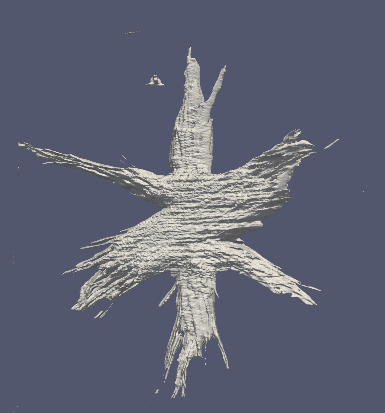
\includegraphics[height=1.35in]{projects/2.3.4-DataViz/2.3.4.13-ECP-VTK-m/VTKm-flying-edges}\quad
  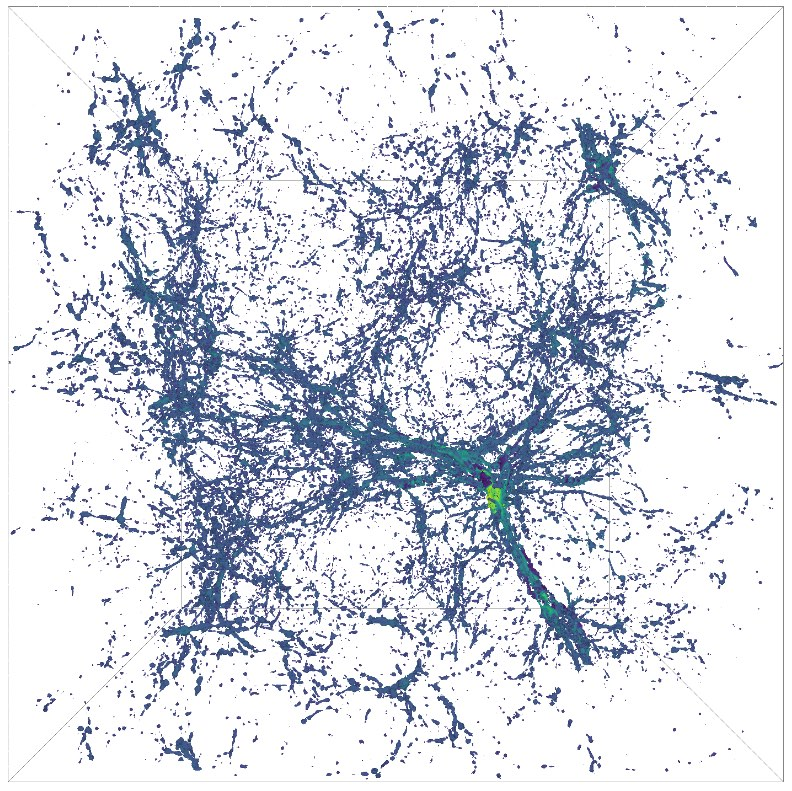
\includegraphics[height=1.35in]{projects/2.3.4-DataViz/2.3.4.13-ECP-VTK-m/VTKm-contour-cell-types}\quad
  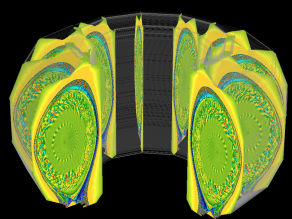
\includegraphics[height=1.35in]{projects/2.3.4-DataViz/2.3.4.13-ECP-VTK-m/VTKm-extruded-cell-set}\quad
  \caption{
    Examples of recent progress in VTK-m include (from left to right) optimized structured grid contouring, contouring of extended cell types, and representation of an extruded cell set.
  }
  \label{fig:VTKmRecent}
\end{figure}

\paragraph{Recent Progress}
The VTK-m project is organized into many implementation activities.
The following features have been completed in the FY20 fiscal year.

\begin{itemize}
\item \textbf{VTK-m Releases:}
  VTK-m 1.5 was released in October 2019.
\item \textbf{Kokkos:}
  Device adapters in VTK-m can now leverage the Kokkos programming model to more rapidly port to ECP hardware.
\item \textbf{Improved Contouring:}
  VTK-m now implements the Flying Edges implementation of structured grid contouring \cite{Schroeder2015}.
  The contouring in VTK-m, demonstrated in Figure \ref{fig:VTKmRecent}, is now measured as one of the fastest implementations in existence.
  VTK-m has also contour support for expanded cell types to support more mesh types, also demonstrated in Figure \ref{fig:VTKmRecent}.
\item \textbf{Data Control Thread Safety:}
  The initial implementation of VTK-m assumed that all control would be on a single thread and all parallelism would be handled internally.
  However, several VTK-m customers need to launch GPU algorithms from multiple different threads.
  The internal management of array data has been redesigned to safely manage data from multiple control threads.
\item \textbf{Spack Package:}
  Spack \cite{Gamblin2015} is the package manager used to distribute the ECP ST software to the ECP platforms.
  The VTK-m package in Spack has been updated to the latest version of VTK-m.
\item \textbf{Random Numbers:}
  Many algorithms rely on pseudo-random numbers.
  VTK-m now uses Salmon, et al's algorithm \cite{Salmon2011} to provide ``random'' arrays that allow algorithms to use numbers with random properties that are correct both within a thread and across threads of execution.
\item \textbf{Extruded Cell Sets:}
  ECP's XGC simulation code uses an extrusion of a surface mesh for its data representation as demonstrated in Figure \ref{fig:VTKmRecent}.
  A similar representation is added to VTK-m for zero-copy data ingestion.
\end{itemize}

\paragraph{Next Steps}
Our next efforts include:

\begin{itemize}
\item \textbf{Demonstrate VTK-m on Pre-Exascale Hardware:}
  With pre-exascale hardware available for O21 (Tulip) and A21 (Iris), VTK-m will be demonstrated on these platforms.
  For FY21 we expect to be able to compile VTK-m, run the regression tests, and use the benchmarking code to compare performance.
\item \textbf{Support New Compiler Types:}
  VTK-m uses CMake to support cross-platform compilation.
  Using CMake with compilers that are not directly supported can be challenging.
  CMake will be updated for new compiler types as necessary, and VTK-m's build system will be similarly updated.
%% \item \textbf{Better Support for Dynamic Types:}
%%   VTK-m (and GPU's in general) prefer knowing static types.
%%   However, it is often not possible to know for sure what specific type data are.
%%   VTK-m's handling of dynmaic types will be improved.
\item \textbf{Resource Management:}
  Add general mechanisms to VTK-m that allow resource management (such as selecting which GPU to use when multiple GPUs are available on a node).
  Providing a general interface prevents code using VTK-m from having to use device-specific API's to control the resource.
\end{itemize}
